% !TEX root = ./main.tex
\graphicspath{{figures_manufactured/}}% Set graphics path location


\subsection{Method of Manufactured Solutions}

\begin{figure}
\centering
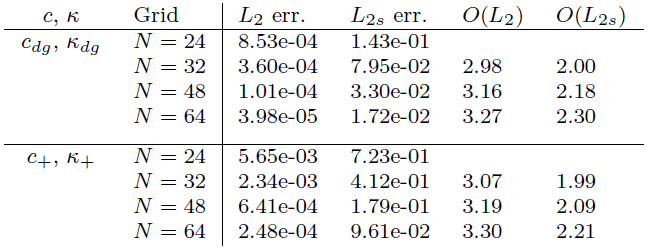
\includegraphics[height=35mm]{table_917} \\
\caption{Accuracy of ESFR schemes for flow generated by a time-dependent source term on triangular grids, for the case of $p = 2$. The inviscid and viscous numerical fluxes were computed using a Rusanov flux with $\lambda = 1$ and a LDG flux with $\tau = 0.1$ and $\beta = \pm 0.5n$.}
\label{fig:table_917}
\end{figure}

\begin{figure}
\centering
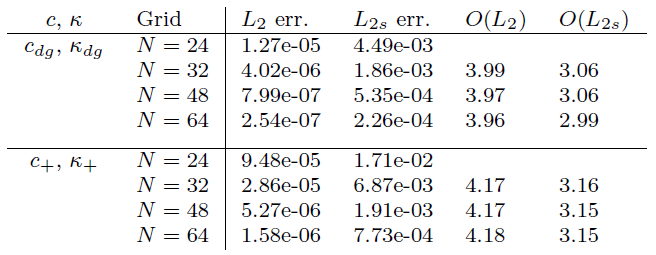
\includegraphics[height=35mm]{table_918} \\
\caption{Accuracy of ESFR schemes for flow generated by a time-dependent source term on triangular grids, for the case of $p = 3$. The inviscid and viscous numerical fluxes were computed using a Rusanov flux with $\lambda = 1$ and a LDG flux with $\tau = 0.1$ and $\beta = \pm 0.5n$.}
\label{fig:table_918}
\end{figure}

\begin{figure}
\centering
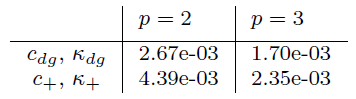
\includegraphics[height=20mm]{table_919} \\
\caption{Explicit time-step limits ($\Delta t_{max}$) of ESFR schemes for flow generated by a time-dependent source term on the triangular grid with $\tilde{N} = 48$, for the cases of $p = 2 and 3$. The inviscid and viscous numerical fluxes were computed using a Rusanov flux with $\lambda = 1$ and a LDG flux with $\tau = 0.1$ and $\beta = \pm 0.5n$.}
\label{fig:table_919}
\end{figure}

\begin{figure}
\centering
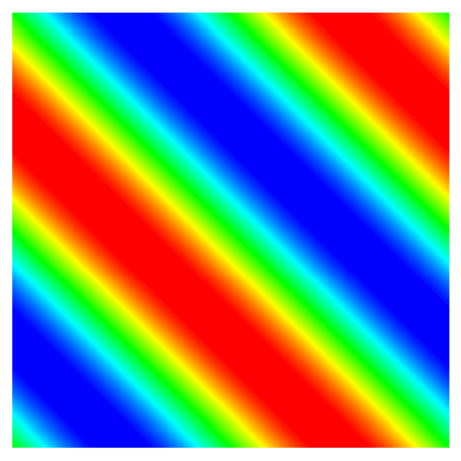
\includegraphics[height=60mm]{figure_912} \\
\caption{Contours of energy obtained using the ESFR scheme with $c = c_+$ and $\kappa = \kappa_+$ on the triangular grid with $\tilde{N} = 32$ for the case of $p = 3$. The inviscid and viscous numerical fluxes were computed using a Rusanov flux with $\lambda = 1$ and a LDG flux with $\tau = 0.1$ and $\beta = \pm 0.5n$.}
\label{fig:figure_912}
\end{figure}

\begin{figure}
\centering
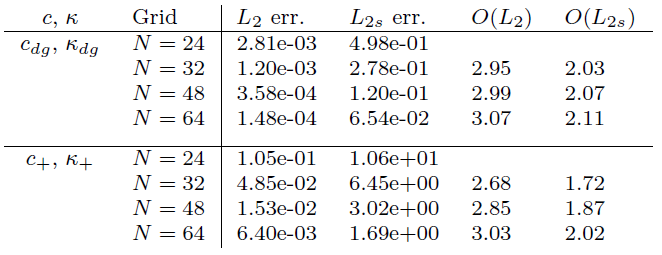
\includegraphics[height=35mm]{table_920} \\
\caption{Accuracy of ESFR schemes for flow generated by a time-dependent source term on tetrahedral grids, for the case of $p = 2$. The inviscid and viscous numerical fluxes were computed using a Rusanov flux with $\lambda = 1$ and a LDG flux with $\tau = 0.1$ and $\beta = \pm 0.5n$.}
\label{fig:table_920}
\end{figure}

\begin{figure}
\centering
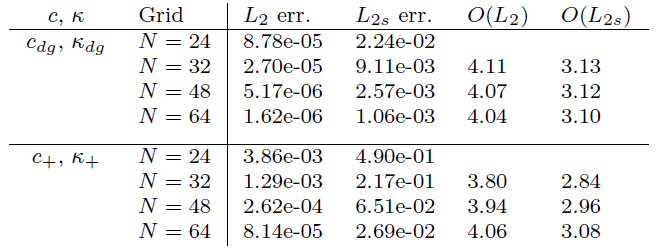
\includegraphics[height=30mm]{table_921} \\
\caption{Accuracy of ESFR schemes for flow generated by a time-dependent source term on tetrahedral grids, for the case of $p = 3$. The inviscid and viscous numerical fluxes were computed using a Rusanov flux with $\lambda = 1$ and a LDG flux with $\tau = 0.1$ and $\beta = \pm 0.5n$.}
\label{fig:table_921}
\end{figure}

\begin{figure}
\centering
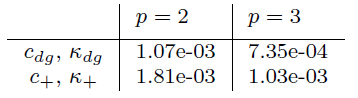
\includegraphics[height=15mm]{table_922} \\
\caption{Explicit time-step limits ($\Delta t_{max}$) of ESFR schemes for flow generated by a time-dependent source term on the triangular grid with $\tilde{N} = 48$, for the cases of $p = 2 and 3$. The inviscid and viscous numerical fluxes were computed using a Rusanov flux with $\lambda = 1$ and a LDG flux with $\tau = 0.1$ and $\beta = \pm 0.5n$.}
\label{fig:table_922}
\end{figure}

\newpage
\begin{figure}
\centering
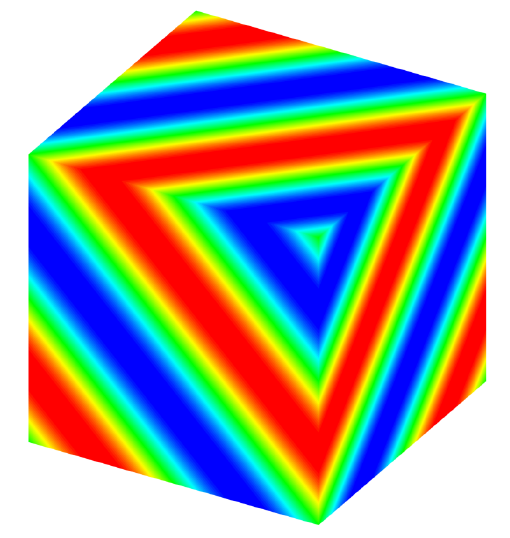
\includegraphics[height=60mm]{figure_913} \\
\caption{Contours of energy obtained using the ESFR scheme with $c = c_+$ and $\kappa = \kappa_+$ on the tetrahedral grid with $\tilde{N} = 32$ for the case of $p = 3$. The inviscid and viscous numerical fluxes were computed using a Rusanov flux with $\lambda = 1$ and a LDG flux with $\tau = 0.1$ and $\beta = \pm 0.5n$.}
\label{fig:figure_913}
\end{figure}
